
\abstract{Resource theories formalize the notion of valuable resources. A quantum resource theory identifies "free states" that can be created with "free operations" - these are "easy" relative to assumed capabilities. To create "resource states", one must either have states that contain "some" of the resource or use resource-generating operations. The theory of entanglement (where the resource is entanglement) and the theory of magic (where the resource is "non-stabilizerness", or "magic") share a similar structure through the lens of resource theory. Our main focus is a particular hierarchical structure of free operations, namely, the gap between the operational definition and the axiomatic definition of these classes of operations. For entanglement, this is the gap between the classes of Local Operations and Classical Communication (LOCC) and Separable Operators. In the case of magic, the gap is between the classes of Stabilizer Operators and Completely Stabilizer Preserving operators. These gaps have potential implications for protocols related to entanglement and magic state distillation.}

\section{Introduction}

The majority of physical theories establish laws based on experimental observations of nature and predict behavior for situations that were not yet verified experimentally. Resource theories in contrast have an inherent process-, or engineering focus as they examine what is possible given a demarcation line in operational capabilities. With roots in Carnot's explorations of how to exploit thermodynamic non-equilibrium as a resource for heat engines, resource theories provide a framework to organize the concepts and questions of availability and quantification of resources, conversion rates, reversibility, and more. At the core of a quantum resource theory, a set of operations is defined to be the \textit{free operations}, or \textit{resource-non-generating} (RNG) operations, and a set of states defined to be the \textit{free states}. The intuition is that RNG operations and free states are the "easy ones", i.e. assumed to be available to acquire without incurring high costs. This is in contrast to valuable \textit{dynamic resources} (resource generating operations), i.e. operations generating \textit{static resources} (resource states) which are "hard" to acquire. \cite{chitambar_quantum_2019}. 

While there are numerous quantum resource theories, the two we are interested in in this report are the theories of entanglement and magic. It is well known that quantum entanglement can be used as a \textit{resource} for communication to extend our capabilities and open up use cases like super-dense coding or quantum teleportation \cite{wilde_quantum_2017}. These use cases would be impossible with the "free" separable states, and \textit{Local Quantum Operations and Classical Communication} (LOCC). 

Magic is a resource for universal fault-tolerant quantum computation (FTQC). Under the stabilizer formalism \cite{gottesman_stabilizer_1997}, large classes of Quantum Error Correction codes can be expressed for both storing and fault tolerantly executing quantum computation in the logical space of these codes. However, stabilizer operations are not universal in the quantum sense, and in-fact are classically efficiently simulatable, as stated by the Gottesman-Knill theorem \cite{gottesman_stabilizer_1997, aaronson_improved_2004}. The term "magic" was introduced in \cite{bravyi_universal_2005}, where Bravyi and Kitaev showed that for universal quantum computation, one has to inject the valuable resource of \textit{magic states} or use non-stabilizer operations.

This report focuses on a particular aspect of resource theories of magic and entanglement, namely, the structure of free operations. Free operations are defined either axiomatically or operationally. The operational definition is usually the more natural, stemming from the assumed limitation on capabilities, and having a clear operational interpretation. Axiomatically defined free operations are more mathematically motivated, they have less clear operational meaning; they are the maximal set of operations that map free states to free states. The question we are interested in is whether the axiomatic class is larger or not than the operational one and if yes, what the implications may be. 

In entanglement theory, the class of separable channels (SEP) are the axiomatically defined free operations and the operational ones are the LOCC operations. Chitambar et al. \cite{chitambar_increasing_2012} found an operationally interpretable measure of entanglement, that shows a 12.5\% gap between SEP and LOCC. In the case of magic theory, a recent counterexample from Heimendahl et al. \cite{heimendahl_axiomatic_2022} shows that the axiomatically defined class of free operations, Completely Stabilizer Preserving (CSP) is strictly larger than the operationally defined class of stabilizer operations (SO). 

The structure of this paper is as follows: in Section \ref{sec:basics} we will cover the minimum prerequisite of notations and concepts to understand the separation of these two classes in these two theories. In Section \ref{sec:free ops} we will then get into the details of the separation of these classes in the two theories and finally, in Section \ref{sec:discussion}, we discuss the potential consequences and draw our conclusions. 

\section{Basics of entanglement and stabilizer theories}\label{sec:basics}

In this section, we review the concepts and mathematical tools in our two theories of interest and establish notation, mostly following Wilde \cite{wilde_quantum_2017} for the quantum information theoretical and entanglement-related concepts. To introduce the stabilizer formalism, we will follow multiple sources  \cite{gottesman_stabilizer_1997, aaronson_improved_2004, heimendahl_axiomatic_2022}. 

\subsection{State vector and density matrix representation of quantum states} 

Quantum mechanics is inherently probabilistic in the sense that measurement outcomes on a system are defined by the amplitude square of a set of complex numbers (\textit{probability amplitudes}) that describe a state as defined by the Born rule. If we can describe the probability amplitudes of a quantum mechanical system with certainty, we call that state a \textit{pure} state. However, this is far from realistic, usually, we don't know perfectly the description of a system. Thus, on top of the inherent "quantum probability distribution", we might have an uncertainty of these amplitudes themselves, layering a "classical probability distribution" over the quantum probability, which we then call \textit{mixed} states (or noisy states). 

Pure quantum states are represented as normalized vectors (or we can think of them as rays) in a potentially composite Hilbert space, i.e. one that allows for a structure of $\mathcal{H}=\otimes_{i=1}^n \mathcal{H}_i$ with each sub-Hilbert space having dimension $d_i$. We will only discuss cases where $d_i = d_j = d, \forall i, j$, i.e. $\mathcal{H}_i=\mathbb{C}^d$, and where $d$ is prime. When $d=2$, we talk about a Hilbert space of $n$ \textit{qubit}s. If $d=3$, we call each subsystem a \textit{qutrit} and $d>3$ is the case of \textit{qudit}s. We denote pure states in the Dirac notation as $\ket{\psi} \in \mathcal{H}$. The members of the computational basis for the $n$ qudit Hilbert space of $d$-dimensional qudits will be labeled by the elements of the vector space $\mathbb{F}_d^n$ over the finite field $\mathbb{F}_d$ (i.e. a $n$ length vector with elements 0 to $d-1$, with addition is modulo $d$).  For example $\ket{124} = \ket{1}\otimes \ket{2} \otimes  \ket{4} \in (\mathbb{C}^5)^{\otimes 3}$ is a 3-qudit state of dimension 5. 

As for mixed states, we don't know exactly which pure state a system is in, we can represent this lack of knowledge as a probability distribution $P_X$ over possible pure states $\ket{\psi_x}$. This ensemble of states and their probabilities $\{(P_X(x), \ket{\psi_x})\}$ affords a \textit{density operator} representation $\rho \equiv \sum_x p_X(x) \ketbra{\psi_x}$, where $\ketbra{\psi_x} \in \mathcal{L}(\mathcal{H})$ is the density operator for the pure state $\ket{\psi_x}$ defined by the outer product of $\ket{\psi_x}$ and $\bra{\psi_x} \equiv \ket{\psi_x}^\dagger$. We denote the set of square linear operators acting on $\mathcal{H}$ with $\mathcal{L}(\mathcal{H})$. A density operator is always positive semi-definite, denoted as $\rho \geq 0$,  and has unit trace, $\Tr\{\rho\}=1$. The set of density operators is denoted as $DO(\mathcal{H}) \subset \mathcal{L}(\mathcal{H})$. 

\subsection{Describing change with operators and quantum channels} 

When the change in a system is noiseless, i.e. the system is closed, it is postulated to be a transformation $U \in \mathcal{L}(\mathcal{H})$ on the system that is \textit{unitary}, i.e. $UU^\dagger=I$. In the vector representation, the effect of $U$ is $\ket{\psi} \rightarrow U\ket{\psi}$, in the density operator formalism, it is $\rho \rightarrow U \rho U^\dagger$. We will make use of the generalizations of the Pauli group, which is generated by the Pauli-X and Pauli-Z operators for a single qubit, with their action on the computational basis:  
\begin{align}
X\ket{k}=\ket{k+1} \ \ ,  Z\ket{k}=(-1)^{k}\ket{k}, k\in \mathbb{F}_2.
\end{align}

The generalized $n$-qudit Pauli-group for $d$ dimension qudits is generated by the generalized $n$-qudit X and Z operators, with action: 

\begin{align}
X(x)\ket{k}=\ket{k+x} \ \ ,  Z(z)\ket{k}=\omega^{k \cdot z}\ket{k}, x,z,k\in \mathbb{F}_d^n.
\end{align}

, where $\omega = e^{i2\pi/d}$ is the $d$th root of unity and $k \cdot z = \sum_{i=1}^{n} k_i z_i$ is the inner product between $k$ and $z$.  

However, in a realistic scenario, evolution is not perfectly known, and as such, it can be thought of as a probabilistic mixture of certain operators. Formally, we represent the most general type of evolution an experimenter can impart on a system with the \textit{quantum channel} formalism. A quantum channel is a map $\mathcal{N}_{A \rightarrow B}: \mathcal{L}(\mathcal{H}_A) \rightarrow \mathcal{L}(\mathcal{H}_B)$, that must map density operators to density operators, i.e. we have to make sure that the output operator $\rho_B := \mathcal{N}_{A \rightarrow B}(\rho_A)$ has trace 1 and is positive. This leads to two mandatory properties. The first property a quantum channel has to satisfy is to be trace-preserving (TP), i.e. $\Tr\{\rho_A\}=\Tr\{\rho_B\}$. The second related to positivity is more subtle, namely that $\rho_B \geq 0$ is not enough, because positivity is not closed under the tensor product. Our map has to be \textit{completely positive} (CP), meaning that for a $\rho_A$ density operator on a system $A$, even if it is extended with an arbitrary reference system $R$ to a density operator $\rho_{AB}$, $(\mathcal{N}_{A \rightarrow B} \otimes id_R) (\rho_{AB}) \geq 0$, i.e. the total system stays positive semi-definite. Both of these properties can be tested via the Choi-Jamiokołwski representation of a channel $\mathcal{E}$:

\begin{align}
J(\mathcal{E}) := (\mathcal{E} \otimes id_n)(\ketbra{\phi^+}),
\end{align}

, where $\ket{\phi^+}:=d^{-n} \sum_{x \in \mathbb{F}_d^n} \ket{xx}$ is the maximally entangled bipartite state on $2n$ $d$-qudits in the computational basis, and $id_n$ is the identity channel acting on the Hilbert space of $n$ $d$-qudits. 
Namely, $\mathcal{E}$ is TP if and only if $Tr(J(\mathcal{E})) = 1$, and $\mathcal{E}$ is CP if and only if $J(\mathcal{E}) \geq 0$. 

We will use the Kraus representation of a quantum channel $\mathcal{E}$, where, for a set of operators called Kraus operators $\{M_i\}$, such that they are \textit{complete}, i.e. $\sum_i M_i^\dagger M_i = I$, the channel's effect is expressed as

\begin{align}
\mathcal{E}(\rho)=\sum_i M_i \rho M_i^\dagger.
\end{align}

Measurement of an \textit{observable} can be described as a quantum channel. An observable $M$ is a Hermitian operator, $M^\dagger=M$, and thus has a spectral decomposition, say $M=\sum_i \lambda_i \ketbra{\phi_i}$, where $\lambda_i \in \mathbb{R}$ are the eigenvalues and $\ket{\phi_i}$ are the corresponding eigenstates. When representing a measurement with this observable, the measurement outcomes are the eigenvalues, and after a certain eigenvalue $\lambda_i$ is observed, the system's state will be projected to the corresponding eigensubspace (of dimension equal to the multiplicity of the eigenvalue), e.g. if $\lambda_i$ has multiplicity 1: $\rho \rightarrow \frac{\ketbra{\phi_i}\rho\ketbra{\phi_i}}{p_M(i)}$, where $p_M(i)=\Tr\{\ketbra{\phi_i}\rho\ketbra{\phi_i}\}$ is the probability of observing $\lambda_i$. 

Finally, we can always find a \textit{Stinespring dilation} of a channel $\mathcal{E}_A$ acting on system $A$, which is a unitary $U_{AR}$ on a larger bipartite system $AR$ such that on the subsystem $A$ its effect (i.e. after tracing out system $R$) is exactly the channel $\mathcal{E}_A$: 

\begin{align}
\mathcal{E}_A(\rho_A) = Tr_B\{ U_{AR}(\rho_A \otimes \ketbra{0}_R) U_{AR}^\dagger \}
\end{align}

, where $\ketbra{0}_R$ is an arbitrary pure state picked from the reference subsystem $R$. 

\subsection{Entanglement} 

A pure quantum state $\ket{\psi}_{AB}$ on a bipartite system $\mathcal{H}_A \otimes \mathcal{H}_B$ is called a \textit{tensor product state} (TPS) or \textit{product state} if it can be expressed as a tensor product of two local states: $\ket{\psi} = \ket{\psi}_A \otimes \ket{\psi}_B$. When there are no states local to the subsystems that can completely describe the state of a pure state, it is \textit{entangled}. A prototypical example is the Bell state, $\frac{\ket{00} + \ket{11}}{\sqrt{2}}$, the qubit case of $\ket{\phi^+}$.

In the case of mixed states, a density operator $\rho$ is called \textit{separable} if it is a convex combination of pure product states, i.e. $\rho = \sum_x p_X(x) \ketbra{\psi_x}_{A} \otimes  \ketbra{\psi_x}_{B}$. We say that a mixed state is \textit{entangled} when it is not separable. The set of separable states is convex, i.e. $\forall \rho, \sigma$ separable, for all $\lambda \in [0,1] : \lambda \rho + (1-\lambda) \sigma$ is also separable.

\subsection{Stabilizer formalism and magic} 

The stabilizer formalism is an efficient way to represent certain subspaces and states in a Hilbert space. For the class of states called \textit{stabilizer states}, which we will define precisely in a moment, simulation and computation with \textit{stabilizer operations} (SO) become classically simulatable. This result is the Gottesman-Knill theorem \cite{gottesman_stabilizer_1997}, and one of its implications is that it identifies a large subset of quantum computing states and operations that are not classical but can be simulated efficiently classically. If one could simulate everything that a quantum computer can do, the field of quantum computing would be in trouble justifying their efforts. Fortunately, this is not the case, as in order to achieve \textit{universality}, one has to use extra resources: either use operations outside of the stabilizer operations or use a generous amount of special states called \textit{magic states}. While we will not need magic states in the later exposition, 
 we remark that Bravyi and Kitaev \cite{bravyi_universal_2005} defined magic states as states that are any Clifford transformations of one of these two types of pure magic states: 

\begin{align*}
\ketbra{T} &= \frac{1}{2}(I + \frac{1}{\sqrt{3}}(X+Z+Y)) \\
\ketbra{H} &= \frac{1}{2}(I + \frac{1}{\sqrt{2}}(X+Z)).
\end{align*}

A state $\ket{\psi} \in \mathcal{H}$ is \textit{stabilized} by an $n$ qudit Hermitian Pauli operator $P \in \mathcal{P}_n(d)$ (Hermiticity is a requirement for it to be an observable) if the state is an eigenstate of it with +1 eigenvalue, i.e $P\ket{\psi} = \ket{\psi}$. For example $\ket{0}$ is stabilized by $Z$ and $\ket{+}$ is stabilized by $X$. 

For two qubits, the situation changes, one might think that for a $\ket{00}$ state, $S_1:=Z_1Z_2$ would be sufficient, however, the +1 eigenspace of $Z_1Z_2$ is two dimensional, both $\ket{00}$ and $\ket{11}$ have +1 eigenvalues. We need then another operator to "filter out" the extra dimension but has $\ket{00}$ as its +1 eigenstate. We find that $S_2:=Z_1I_2$ is a good example. We can also notice that $S_1S_2 = I_1Z_2$, which is also a stabilizer for $\ket{00}$, and naturally $I_1I_2$ is also a stabilizer. The set $\{S_1, S_2, S_1S_2, I\}$ is a \textit{group}, that is closed under operator multiplication. Also, all of its members commute with each other (i.e. it's \textit{Abelian}), thus they can be diagonalized simultaneously. Their shared +1 eigenspace is the \textit{stabilized subspace}. 

In general, we can represent an Abelian group of size $2^k$ with only $k$ independent elements, the \textit{generators}. An Abelian subgroup of the $n$-qudit Pauli group is called a \textit{stabilizer group} if it does not contain the element $- \mathbb{I}$ (to ensure that all stabilizers are Hermitian). As each generator "halves" the Hilbert space, we can see that a $k$ dimensional stabilizer group stabilizes an $n-k$ dimensional subspace. When $n=k$, we have a \textit{stabilizer state}. Single qubit stabilizer states are:

\begin{align*}
Z: \ket{0} \ -Z: \ket{1} \\
X: \ket{+} \ -X: \ket{-} \\
Y: \ket{i} \ -Y: \ket{-i}
\end{align*}

, also $I$ stabilizes all states, and $-I$ stabilizes no states. For two-qubit states, $XX,ZZ$ stabilizes the Bell state, and in general, $\ket{\phi^+}$ is a stabilizer state. The set of $n-qubit$ stabilizer states is denoted as $STAB_n(2)$. Convex combinations of stabilizer states are \textit{mixed stabilizer states}, and they form \textit{stabilizer polytope}, denoted $SP_n(2):=convex(STAB_n(2))$. In the single qubit case, this is a simple octahedron on the Bloch sphere as displayed in Figure \ref{fig:stab_polytope}. 

\begin{figure}[!ht]
\center
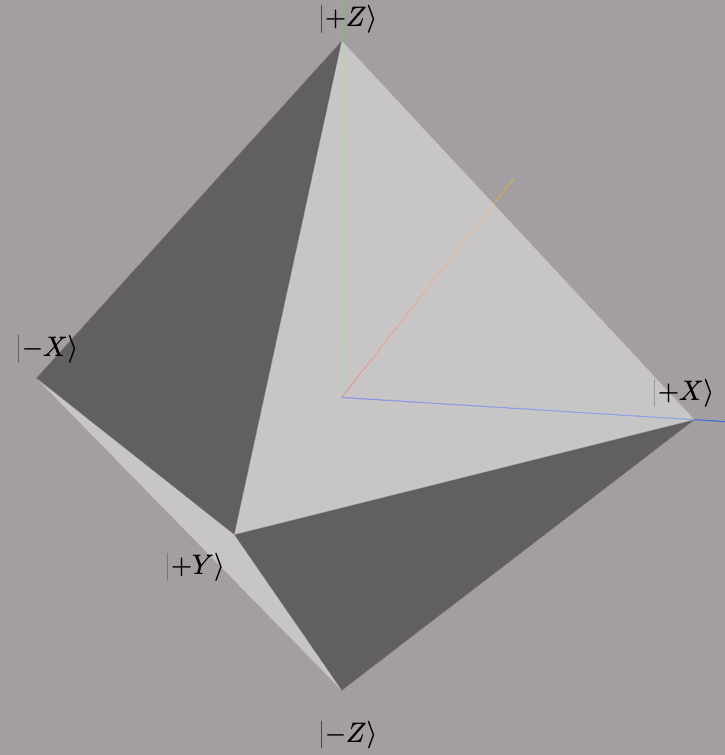
\includegraphics[scale=.3]{stab_polytope.png}
\caption{The stabilizer polytope for single qubit stabilizer states. In higher dimensions, the polytope is more complex.}
\label{fig:stab_polytope}
\end{figure}


An $n$-qubit Pauli operator can be represented by $2n+1$ bits, with 2 bits for each qubit for the choice of $X=10, Z=01, Y=11, I=00$ and 1 bit for the global phase, the sign $\pm$. Thus a stabilizer state can be described by $n$ $n$-qubit Pauli operators, and as such it requires only $2n^2 + n=O(n^2)$ bits. This polynomial cost is in sharp contrast with the $2^n$ complex numbers required to represent a general state. 

Beyond the efficient representation of states, it is possible to efficiently update the state if we limit the set of operations to those that map stabilizer states to stabilizer states. As an $n$-qubit stabilizer state can be represented by $n$ $n$-qubit Pauli operators, we need these operators to map Pauli operators to Pauli operators. The largest set of unitary operators that satisfy this criterion is the Clifford group, $Cl_n(2)$, generated by the $H$, $CNOT$, and the $S=\sqrt{Z}$ gates. Gottesman and Knill showed that a polynomial number of operations is sufficient to simulate Clifford operations or Pauli measurements.

\section{The structure of free operations}\label{sec:free ops}

In this section, we will review how the structure of free operations has a gap between axiomatic and operational definitions. In the case of entanglement, after a quick descriptive example for separation from Bennett et al. \cite{bennett_quantum_1999}, we follow Chitambar et al. \cite{chitambar_increasing_2012} and for magic, the work by Heimendahl et al.  \cite{heimendahl_axiomatic_2022}. 

\subsection{Entanglement: $LOCC \subset SEP$}

As mentioned before, in entanglement theory, the operational and axiomatic classes of RNG operations are the LOCC and the Separable (SEP) channels. 
\begin{definition}\textit{A channel $\mathcal{E}$ on a Hilbert space of $N$ qudits is a \textbf{separable channel} if it has a Kraus decomposition with separable Kraus operators, i.e.: 
\begin{align}
\mathcal{E}(\rho) = \sum_l A_l \rho A_l^\dagger, A_l = M_{1,i} \otimes M_{2,i} \otimes \ldots \otimes M_{N,i}.
\end{align}}

The set of separable channels is denoted SEP.
\end{definition}
                  
An early example by Bennett et al. \cite{bennett_quantum_1999} shows the separation between these two classes, which shows "non-locality without entanglement". In Figure \ref{fig:dominos} we can see 9 states in a domino notation. Alice and Bob both have a qutrit and they can be in one of the 9 states. They are each a bipartite, separable state and mutually orthogonal to each other. However, in order to distinguish them, one has to do a non-local measurement. To create the states we have to use Separable channels. Let $\ket{\psi_i}$ denote the 9 states. Then, the measurement that can distinguish these states can be represented by the Kraus representation $S(\rho)=\sum_i S_i \rho S_i^\dagger$, where: 
\begin{align}
S_i = \ket{i}_A \ket{i}_B\bra{\psi_i}. 
\end{align}

\begin{figure}[!ht]
\center
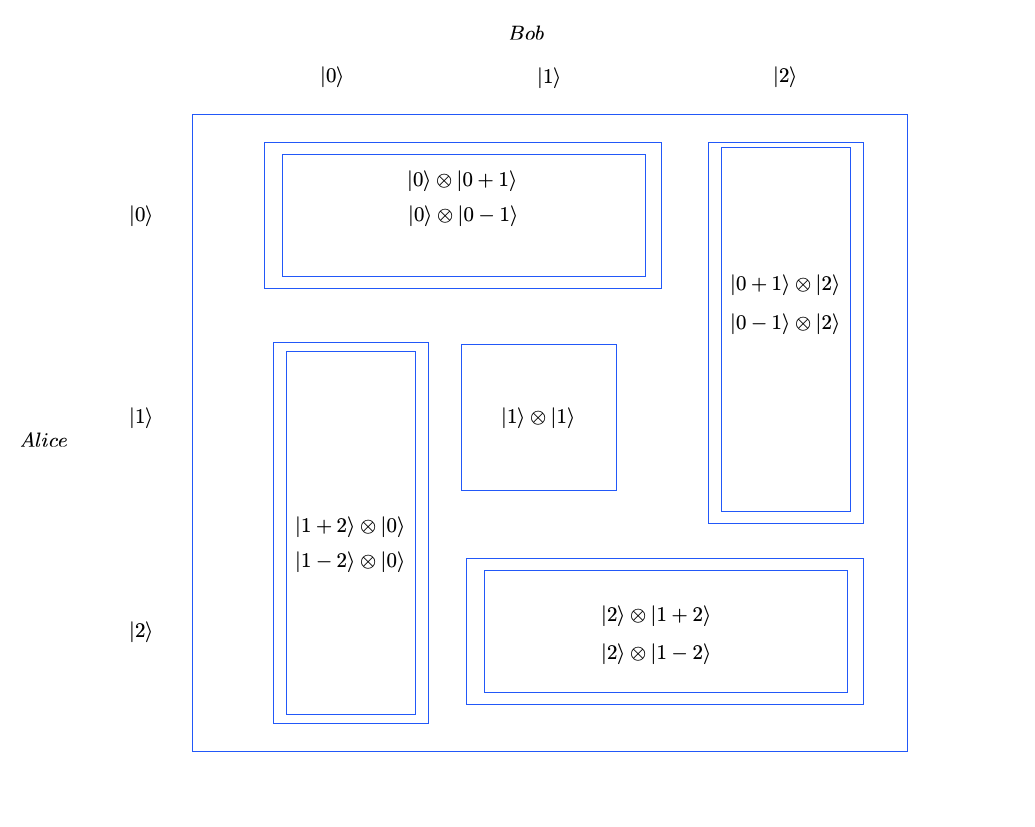
\includegraphics[scale=.4]{dominos.png}
\caption{The 9 orthogonal states on the two-qutrit Hilbert space are all separable but only distinguishable by non-local measurements, and  indistinguishable locally.}
\label{fig:dominos}
\end{figure}

An intuition around how local measurements would act here is that they would always "cut" at least one of the dominoes "in half", which would make those states indistinguishable. It is laboriously derived and carefully argued in  \cite{bennett_quantum_1999} that this measurement operator cannot be implemented by LOCC operations (however, it can be prepared locally!), on the other hand, it is clearly a separable channel. Thus, $LOCC \subset SEP$. 

The seminal work from Bennett et al. also quantified the gap, but only to the order of $10^{-6}$. A central objective of the approach by \cite{chitambar_increasing_2012} was to quantify this gap and define a measure of entanglement that can have a significant difference between the two classes. They managed to show a 12.5\% gap using a measure that also has an operational interpretation. 

\begin{definition} \textit{Suppose we have an arbitrary state $\rho \in DO(\mathcal{H})$, and a set of LOCC transformations, each executed with probability $p_i$, converting $\rho$ into $\rho_i$. Then, we call a function $\mu: DO(\mathcal{H}) \rightarrow \mathbb{R}$ an \textbf{entanglement monotone}, when it satisfies the following inequality: 
\begin{align}
\mu(\rho) \leq \sum_i p_i \mu(\rho_i)
\end{align}
}
\end{definition}

Chitambar et al. defined a monotone that measures the success rate of a particular task: random-EPR pair distillation from  W-class states. W-class states are any state that is obtainable from the $\ket{W}=\frac{1}{\sqrt{3}}(\ket{100}+\ket{010}+\ket{001})$ state with LOCC operations and can be parameterized as $\sqrt{x_0}|000\rangle + \sqrt{x_A}|100\rangle + \sqrt{x_B}|010\rangle + \sqrt{x_C}|001\rangle$. Due to normalization $x_0$ is fully determined by $1=x_0+x_A+x_B+x_C$, thus we will label W-class states as $\vec{x}=\{x_A,x_B,x_C\}$. In random-EPR pair distillation, one uses a protocol to transform an initial W-class state to random singlet states $\ket{\psi}_ij=\frac{1}{\sqrt{2}}(|01\rangle_{ij} + |10\rangle_{ij})$ between any two of the 3 parties as shown in Figure \ref{fig:epr}.

\begin{figure}[!ht]
\center
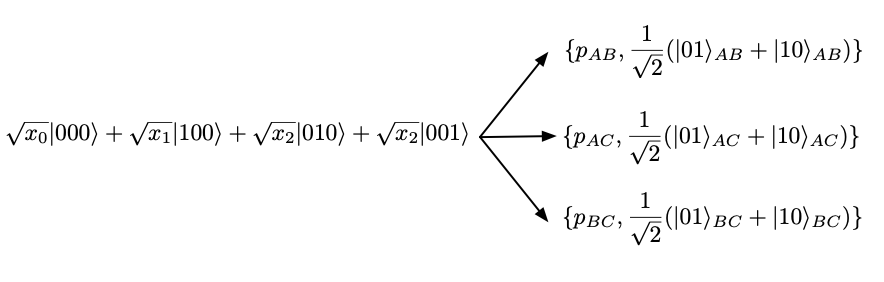
\includegraphics[scale=.4]{epr.png}
\caption{Random-EPR pair distillation from a W-class state.}
\label{fig:epr}
\end{figure}

For  $\vec{x}=\{x_A,x_B,x_C\}$, let $\{n_1,n_2,n_3\}$ be a labeling of $\{A,B,C\}$ so that $x_{n_1} \geq x_{n_2} \geq x_{n_3}$. Then, the function 
\begin{align}
\kappa(\vec{x}) := 2(x_{n_2} + x_{n_3}) - \frac{x_{n_2}x_{n_3}}{x_{n_1}} 
\end{align}

is an entanglement monotone that strictly decreases on average when a party with maximum component value makes a measurement by Theorem 1 in \cite{chitambar_increasing_2012}. 

The function $\kappa(\vec{x})$ can reach 1 if and only if $x_{n_1}=x_{n_2}$ and $x_0=0$, and thus $p_{AB}+p_{BC}+p_{AC}\leq \kappa(\vec{x})$ for any $\vec{x}$ - thus we have an upper bound on the total probability of the success rate for the random-EPR distillation of $\vec{x}$. Interestingly, by Theorem 2. in \cite{chitambar_increasing_2012}, for a class of $x_{n_3} > x_0=0$ states, the success rate of LOCC operations can get arbitrarily close to this bound, for any $\epsilon>0$, $p_{AB}+p_{BC}+p_{AC}>\kappa(\vec{x})-\epsilon$, but no LOCC operation can exactly reach $\kappa(\vec{x})$. 

The situation is different for SEP channels as there exists a set of separable measurement operators that can randomly distill a three-qubit W-class state with $x_0=0, 1/2 \geq x_A \geq x_B \geq x_C$ with probability one:

\begin{align}
M_{AB} &= (\lambda_{CB} \ketbra{0} + \ketbra{1}) \otimes (\lambda_{CA} \ketbra{0} + \ketbra{1}) \otimes \ketbra{0} \\
M_{AC} &= (\lambda_{BC} \ketbra{0} + \ketbra{1}) \otimes \ketbra{0} \otimes (\lambda_{BA} \ketbra{0} + \ketbra{1}) \\
M_{BC} &= \ketbra{0} \otimes (\lambda_{AC} \ketbra{0} + \ketbra{1}) \otimes  (\lambda_{AB} \ketbra{0} + \ketbra{1}) \\
M_{000} &= (1-\lambda_{CA}^2\lambda_{CB}^2-\lambda_{BA}^2\lambda_{BC}^2-\lambda_{AB}^2\lambda_{AC}^2)^{1/2}\ketbra{000} \\
M_{111} &= \ketbra{111}
\end{align}

, where $\lambda_{ij}=\sqrt{\frac{1-2x_i}{2x_j}}$.

The example where the 12.5\% difference shows up is the following family of states parameterized by $\frac{1}{3} \leq s \leq \frac{1}{2}$:

\begin{align}
\sqrt{s} \ket{100} + \sqrt{\frac{1-s}{2}}(\ket{010}+\ket{001}) \label{eq:param-w-class}
\end{align}

While the SEP probability is 1, the LOCC probability is bound by $\kappa(\vec{x}) = 2(1-s)-\frac{(1-s)^2}{4}$. We plot the two functions in Figure \ref{fig:kappas}, where the separation is clearly visible. 

\begin{figure}[!ht]
\center
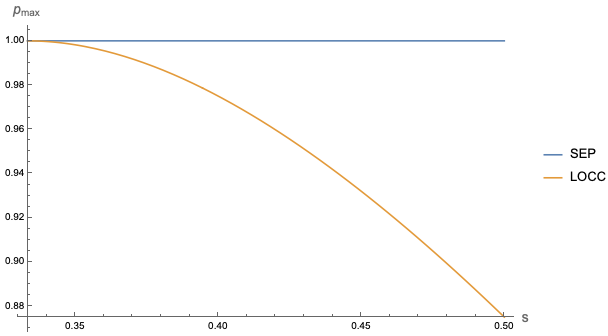
\includegraphics[scale=.4]{kappas.png}
\caption{Maximum probability of generating EPR pairs from a parameterized W-class state defined in \ref{eq:param-w-class}.}
\label{fig:kappas}
\end{figure}


\subsection{Stabilizer formalism: $SO_n(d) \subset CSP$ }

The operationally defined set of free operations in the stabilizer formalism is the Stabilizer Operators. We will formally define them here. All the above concepts in Section \ref{sec:basics} including the Pauli group $\mathcal{P}_n(d)$, the stabilizer group $S$, the Clifford group $Cl_n(d)$, and stabilizer states STAB($d,n$) readily generalize from qubits to qudits as described in  \cite{heimendahl_axiomatic_2022}. Our formal definitions then will be stated using qudits: 

\begin{definition} 
\textit{A quantum channel mapping $n$ $d$-qudits to $m$ $d$-qudits, for prime dimension $d$, is defined as a \textbf{Stabilizer operation} when it is a concatenation of operations that fall into one of the following categories:
\begin{itemize}
\item preparation of qudits in stabilizer states 
\item application of a Clifford unitary
\item measurement of a Pauli observable
\item discarding of qudits
\end{itemize}
Beyond the above, arbitrary random functions of previous measurement results can act as classical logic to decide which quantum operation to do in each step. 
}
\end{definition} 

We are taking the stabilizer polytope for $n$-qudits of $d$ dimension, $SP_n(d)$ to be the set of free states. Then, the axiomatically defined RNG operations are the ones that map the stabilizer-polytope to itself. Similar to positivity, in some resource theories, these channels are not closed under tensor product. In order to enforce closeness under tensor product, the set of \textit{completely}-RNG channels are of interest - in our case the Completely Stabilizer Preserving (CSP) channels, which - for any arbitrary $k$ dimensional extension, maps the $n+k$ dimensional stabilizer polytope to the $m+k$ dimensional stabilizer polytope: 

\begin{definition}
\textit{A linear superoperator $\mathcal{E}$ mapping $n$ and $m$ qudit spaces of $d$ dimension is \textbf{Completely Stabilizer Preserving} if and only if $\mathcal{E} \otimes id_k (SP_{n+k}(d)) \subset SP_{m+k}(d)$ for all $k \in \mathbb{N}$.  }
\end{definition}

A CSP operator is also CPTP \cite{heimendahl_axiomatic_2022}, thus they are legitimate quantum channels. How can we determine whether a stabilizer-preserving channel $\mathcal{E}$ is also CSP? An interesting result \cite{seddon_quantifying_2019} utilizes the Choi operator to prove that if the Choi operator (which can be looked at as a state) of $\mathcal{E}$ is stabilizer-preserving and trace-preserving, then $\mathcal{E}$ is CSP. 

With the definitions out of the way, let's look at the main result by Heimendahl et al. For the single qudit (qubit) case, $SO_1(d)= CSP_1(d)$. This is intuitively reasonable, as  However, starting from two qubits, CSP is strictly larger than SO. Heimendahl et al used the following channel as a counterexample to prove the separation between $SO_2(2)$ and $CSP_2(2)$: 

\begin{align}
\Lambda(\rho) = \rho_{00} \ketbra{++} + \sum_{x \in \{01, 10, 11\}} \rho_{x,x} \ketbra{x} + \frac{1}{2} \sum_{\substack{x,y \in \{01, 10, 11\} \\ x\neq y}} \rho_{x,y}\ket{x}\bra{y}
\end{align}

, where $\rho_{x,y}=\bra{x} \rho \ket{y}$. 

This channel can be written as the following three operations:
\begin{enumerate}
\item  measure a projective measurement that distinguishes between $\ket{00}$ and the subspace spanned by $\ket{01},\ket{10},\ket{11}$, i.e. $\ket{00}^\perp$. This operation cannot be implemented using stabilizer operations. This makes the density matrix block-diagonal: 
\begin{align}
\begin{pmatrix}
\rho_{00} & 0 & 0 & 0 \\
0 & \rho_{01,01} & \rho_{01,10} & \rho_{01,11} \\
0 & \rho_{10,01} & \rho_{10,10} & \rho_{10,11} \\
0 & \rho_{11,01} & \rho_{11,10} & \rho_{11,11} 
\end{pmatrix}
\end{align}
\item Apply partial dephasing with probability 1/2. Off-diagonal terms become half their size: 
\begin{align}
\begin{pmatrix}
\rho_{00} & 0 & 0 & 0 \\
0 & \rho_{01,01} & \rho_{01,10}/2 & \rho_{01,11}/2 \\
0 & \rho_{10,01}/2 & \rho_{10,10} & \rho_{10,11}/2 \\
0 & \rho_{11,01}/2 & \rho_{11,10}/2 & \rho_{11,11} 
\end{pmatrix}
\end{align}
\item Depending on the outcome of the measurement, apply Hadamard on both qubits if $\ket{00}$ was observed. At this point, we get the expression for $\Lambda(\rho)$. 
\end{enumerate}

It is possible to show that all three steps are necessary for the channel to be CSP but not SO. In a bit more intuitive explanation, in the geometry of the space of channels, after the first step, we are outside of the CSP class (which is also a polytope). The dephasing step removes sufficient "magic" from the channel to make it CSP and the Hadamard at the end sets the direction the CSP polytope is being approached from to make the channel a vertex. 

We will introduce the notion of a Clifford dilation for the sketch of the proof. 
A superoperator $\mathcal{E}$ mapping $n$ and $m$ qudit spaces of $d$ dimension has a Clifford dilation if there exists a number $k$, a stabilizer state $\ket{s} \in SP_k(d)$ and a Clifford unitary $U$ on $n+k$ qudits such that: 
$$
\mathcal{E}(\rho) = Tr_{m+1,...n+k}\{U(\rho \otimes \ketbra{s})U^\dagger\}
$$

The channels that have a Clifford dilation are the ones that have no measurements or classical randomness.

The sketch of the proof is the following: 
\begin{enumerate}
\item it is shown that $\Lambda$ is an \textit{almost-diagonal channel}, meaning that it belongs to $AD_2$ that is defined by its effect on the computational basis states: 
\begin{align}
\mathcal{E}(\ketbra{00})=\ketbra{++}, \mathcal{E}(\ketbra{x})=\ketbra{x}, x \in \ket{00}^\perp
\end{align}
\item This property is then used to show that $\Lambda$ is extremal in $CS_2$. From here, if $\Lambda$ is a stabilizer operation, then it would follow that it is an extremal point in $SO_2$ as well. This is due to convex subsets inheriting the extremality of points from their supersets. 
\item It is shown that extremal points in $SO_2$ do not have a Clifford dilation.
\item However, it can be proved that $\Lambda$ cannot have a Clifford dilation - thus it must be that $\Lambda \in CSP_2$ but $\Lambda \notin SO_2$
\end{enumerate}

For larger qubit and qudit dimensions we refer the reader to \cite{heimendahl_axiomatic_2022}. For the full picture though, it is worth mentioning that for larger dimensional qudit states even $CSP_n(d)$ might not be maximal in terms of free operations. For $d$ odd dimensions, resource theories of magic use the Wigner function representation of a function. This is a quasi-probability distribution in phase-space and its total negativity is a magic monotone called \textit{mana}. Thus, the set of free states can be enlarged to include those with positive Wigner functions, and channels that preserve the positivity of the Wigner function and do so closed under the tensor product are called the \textit{completely}-Wigner-positivity-preserving ($CWPP_n,m(d)$) channels. Thus in case of odd $d>2$ dimensions, the full hierarchy is $SO_{n,m}(d) \subset CSP_{n,m} \subseteq CWPP_{n,m}(d)$, where the last containment is conjectured to be proper by Heimendahl et al. 

\section{Discussion}\label{sec:discussion}

Starting from the basics, we reviewed how the structure of the free operations in the theories of entanglement and magic are structured.  To explore entanglement, we looked at an early example by Bennett et al. that demonstrated measurement that is separable but not LOCC. Following Chitambar et al., we explored an entanglement monotone specifically designed to measure the maximum success of random-EPR distillation from W-class states, and how it can show a 12.5\% gap between LOCC and SEP. 

For the theory of magic, Heimendahl et al. did not work with magic monotones, instead, for 2-qubit states, they showed through a specific counter-example that is a completely stabilizer preserving operation but not a stabilizer operation. One could say that their result is similar in spirit to the Bennett et al. example, where careful arguments around a specific set of counterexamples demonstrate the separation of the two classes. Future work might explore actually quantifying the gap in this theory as well for magic distillation tasks. Further implications of the CSP / SO separation could be that the classically simulatable class of channels will become larger, beyond the Gottesman-Knill theorem. 
